%% fair-publish — Technical demo presentation
%% Companion to CRIS2026 paper #23

\documentclass[aspectratio=169]{beamer}

\usepackage{hyperref}
\usepackage{url}
\usepackage{tikz}
\usetikzlibrary{arrows.meta, positioning, shapes, fit, backgrounds}
\usepackage{listings}
\usepackage{xcolor}

%------------------------------------------------------------------------------
% Color palette (UAH brand)
%------------------------------------------------------------------------------
\definecolor{crisnavy}{HTML}{00288C}
\definecolor{cristeal}{HTML}{1A4DAF}
\definecolor{crislight}{HTML}{D6E4F7}
\definecolor{crisaccent}{HTML}{5585CC}
\definecolor{crisgray}{HTML}{3E3E3E}
\definecolor{crisgreen}{HTML}{2E7D32}
\definecolor{crisred}{HTML}{C62828}

%------------------------------------------------------------------------------
% Listings style
%------------------------------------------------------------------------------
\lstdefinestyle{yaml}{
  language=,
  basicstyle=\ttfamily\tiny,
  keywordstyle=\color{cristeal}\bfseries,
  stringstyle=\color{crisgreen},
  commentstyle=\color{crisgray}\itshape,
  showstringspaces=false,
  frame=single, framerule=0.4pt, rulecolor=\color{crisaccent},
  backgroundcolor=\color{crislight!40},
  breaklines=true, columns=fullflexible,
}
\lstdefinestyle{python}{
  language=Python,
  basicstyle=\ttfamily\tiny,
  keywordstyle=\color{cristeal}\bfseries,
  stringstyle=\color{crisgreen},
  commentstyle=\color{crisgray}\itshape,
  showstringspaces=false,
  frame=single, framerule=0.4pt, rulecolor=\color{crisaccent},
  backgroundcolor=\color{crislight!40},
  breaklines=true, columns=fullflexible,
}
\lstdefinestyle{shell}{
  language=bash,
  basicstyle=\ttfamily\tiny,
  keywordstyle=\color{crisnavy}\bfseries,
  stringstyle=\color{crisgreen},
  commentstyle=\color{crisgray}\itshape,
  showstringspaces=false,
  frame=single, framerule=0.4pt, rulecolor=\color{crisaccent},
  backgroundcolor=\color{crisgray!8},
  breaklines=true, columns=fullflexible,
}

%------------------------------------------------------------------------------
% Beamer theme
%------------------------------------------------------------------------------
\usetheme{default}
\usecolortheme{default}
\usefonttheme{professionalfonts}

\setbeamercolor{frametitle}{bg=crisnavy, fg=white}
\setbeamercolor{title}{fg=crisnavy}
\setbeamercolor{structure}{fg=crisnavy}
\setbeamercolor{block title}{bg=cristeal, fg=white}
\setbeamercolor{block body}{bg=crislight, fg=crisgray}
\setbeamercolor{alerted text}{fg=cristeal}
\setbeamercolor{itemize item}{fg=cristeal}
\setbeamercolor{itemize subitem}{fg=crisnavy}
\setbeamercolor{footline}{bg=crisnavy, fg=white}
\setbeamertemplate{navigation symbols}{}

\addtobeamertemplate{frametitle}{}{%
  \begin{tikzpicture}[remember picture, overlay]
    \node[anchor=north east, inner sep=4pt]
      at (current page.north east)
      {
\includegraphics[height=0.52cm]{uah-logo-white.png}};
  \end{tikzpicture}%
}
\setbeamertemplate{itemize item}{\small\raisebox{0.5pt}{\textcolor{cristeal}{$\blacktriangleright$}}}
\setbeamertemplate{itemize subitem}{\small\raisebox{0.5pt}{\textcolor{crisnavy}{$\bullet$}}}
\setbeamertemplate{footline}{%
  \begin{beamercolorbox}[wd=\paperwidth, ht=2.5ex, dp=1.5ex]{footline}%
    \hspace{1em}\textbf{fair-publish} --- Technical overview%
    \hfill University of Alcalá / IRyCIS%
    \hfill\insertframenumber\,/\,\inserttotalframenumber\hspace{1em}%
  \end{beamercolorbox}%
}

%------------------------------------------------------------------------------
\title{\texttt{fair-publish}}
\subtitle{Policy-enforced FAIR metadata validation and publishing pipeline\\[4pt]
  \normalsize Technical overview \& demo}
\author{M.-A. Sicilia · A. Ballesteros-Rodríguez · E. García-Barriocanal ·
  M. Mora-Cantallops · A. Nogales}
\institute{University of Alcalá \textbar{} IRyCIS}
\date{}

%------------------------------------------------------------------------------
\begin{document}
%------------------------------------------------------------------------------

\begin{frame}[plain]
  \vspace{1.2cm}
  \begin{tikzpicture}[remember picture, overlay]
    \fill[crisnavy] (current page.north west) rectangle +(\paperwidth,-1.1cm);
    \fill[cristeal] (current page.south west) rectangle +(\paperwidth,1.2cm);
    \node[anchor=west, inner sep=6pt]
      at ([yshift=0.6cm]current page.south west)
      {
\includegraphics[height=0.9cm]{uah-logo-white.png}};
  \end{tikzpicture}
  \titlepage
\end{frame}

\begin{frame}{Outline}
  \tableofcontents
\end{frame}

%==============================================================================
\section{What problem does it solve?}
%==============================================================================

\begin{frame}{The metadata publication problem}
  \begin{columns}[T]
    \column{0.52\textwidth}
      In a research organisation, a dataset record must be:
      \begin{itemize}
        \item Described in a \textbf{Data Management Plan} (DMP)
        \item Validated against \textbf{institutional policy}
        \item Published to \textbf{one or more FAIR repositories}
        \item \textbf{Versioned} when the dataset evolves
      \end{itemize}
      \vspace{0.35cm}
      Today this is done \alert{manually, inconsistently, and late}
    \column{0.45\textwidth}
      \begin{block}{The CI/CD analogy}
        Software engineering solved the same problem:\\[4pt]
        \textbf{source of truth} (code) $\to$ \textbf{automated tests}
        (policy) $\to$ \textbf{release} (repository)\\[6pt]
        \texttt{fair-publish} applies this pattern to\\
        \textbf{FAIR metadata publication}
      \end{block}
  \end{columns}
\end{frame}

%==============================================================================
\section{Architecture}
%==============================================================================

\begin{frame}{System architecture}
  \begin{center}
  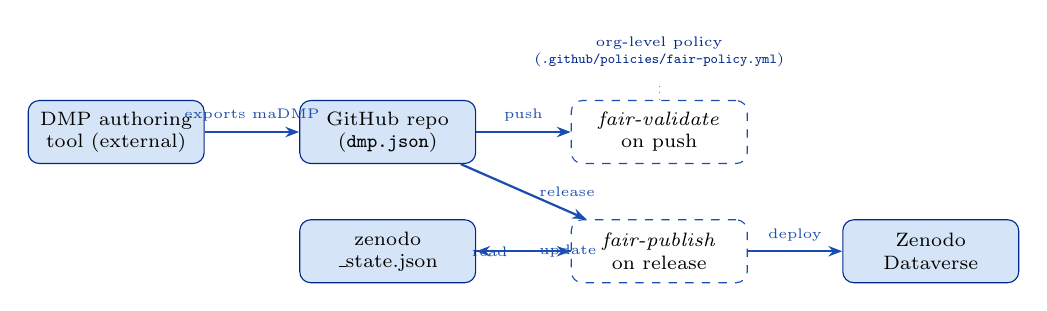
\begin{tikzpicture}[
    font=\scriptsize,
    node distance=0.5cm and 0.8cm,
    box/.style={draw=crisnavy, fill=crislight, rounded corners=4pt,
                text width=2.0cm, align=center, minimum height=0.8cm},
    store/.style={draw=cristeal, fill=white, rounded corners=4pt,
                  text width=2.0cm, align=center, minimum height=0.8cm, dashed},
    arr/.style={-{Stealth[length=5pt]}, cristeal, thick},
  ]
    \node[box] (tool)  {DMP authoring\\tool (external)};
    \node[box, right=1.2cm of tool] (gh)   {GitHub repo\\(\texttt{dmp.json})};
    \node[store, right=1.2cm of gh]  (gha1) {\textit{fair-validate}\\on push};
    \node[store, below=0.7cm of gha1](gha2) {\textit{fair-publish}\\on release};
    \node[box, right=1.2cm of gha2]  (zen)  {Zenodo\\Dataverse};
    \node[box, below=0.7cm of gh]    (state){zenodo\\\_state.json};

    \draw[arr] (tool) -- node[above,font=\tiny]{exports maDMP} (gh);
    \draw[arr] (gh)   -- node[above,font=\tiny]{push} (gha1);
    \draw[arr] (gh)   -- node[right,font=\tiny,xshift=2pt]{release} (gha2);
    \draw[arr] (gha2) -- node[above,font=\tiny]{deploy} (zen);
    \draw[arr] (gha2) -- node[right,font=\tiny,xshift=2pt]{update} (state);
    \draw[arr] (state) -- node[left,font=\tiny,xshift=-2pt]{read} (gha2);

    % Org policy annotation
    \node[above=0.3cm of gha1, font=\tiny, crisnavy, align=center]
      {org-level policy\\(\texttt{.github/policies/fair-policy.yml})};
    \draw[crisaccent, dotted] (gha1.north) -- ++(0, 0.25);
  \end{tikzpicture}
  \end{center}
\end{frame}

\begin{frame}{Two-workflow design}
  \begin{columns}[T]
    \column{0.48\textwidth}
      \textbf{Workflow 1: \texttt{fair-validate.yml}}\\
      \textit{Trigger: push / pull request to main}
      \begin{itemize}
        \item Structural validation via \texttt{madmpy}
        \item Policy rule checks (per dataset)
        \item Blocks merge if any error-level rule fails
        \item Writes GHA step summary with rule-by-rule table
      \end{itemize}
      \vspace{0.3cm}
      \begin{alertblock}{Governance requirement}
        \footnotesize Branch protection rules must require this
        workflow to pass --- otherwise a PI can release without
        validation
      \end{alertblock}

    \column{0.48\textwidth}
      \textbf{Workflow 2: \texttt{fair-publish.yml}}\\
      \textit{Trigger: GitHub release published}
      \begin{itemize}
        \item Publishes each dataset in the DMP to Zenodo
        \item New dataset $\to$ new Zenodo record
        \item Known dataset $\to$ new version (via \texttt{zenodo\_state.json})
        \item Commits updated state file back to repo
        \item Creates \texttt{published/<tag>} git tag
      \end{itemize}
  \end{columns}
\end{frame}

%==============================================================================
\section{The rule system}
%==============================================================================

\begin{frame}[fragile]{Built-in FAIR rules}
  Rules operate on \texttt{(DMP, Dataset)} pairs from \texttt{madmpy} objects.

  \vspace{0.3cm}
  \begin{columns}[T]
    \column{0.48\textwidth}
      \textbf{Built-in rules:}
      \begin{itemize}
        \item Creator ORCID present \hfill\textit{F1, A1}
        \item License present \& recognized \hfill\textit{R1.1}
        \item At least one keyword \hfill\textit{F2}
        \item Description $\geq$ N chars \hfill\textit{F2, R1}
        \item Access rights stated \hfill\textit{A1}
        \item Dataset identifier present \hfill\textit{F1}
      \end{itemize}
      \vspace{0.2cm}
      Each rule returns:\\
      \texttt{passed}, \texttt{severity}, \texttt{field}, \texttt{message}, \texttt{fair}

    \column{0.50\textwidth}
      \begin{lstlisting}[style=python, caption={Rule protocol}]
class Rule(Protocol):
    name: str
    severity: str  # "error" | "warning"
    fair: str

    def __call__(
        self, dmp: Any, dataset: Any
    ) -> RuleResult: ...
      \end{lstlisting}
      \vspace{0.15cm}
      \footnotesize \textbf{error} $\to$ blocks publishing\\
      \textbf{warning} $\to$ reported only
  \end{columns}
\end{frame}

\begin{frame}[fragile]{Custom domain rules}
  Institutions add domain-specific rules without modifying the core package.

  \begin{columns}[T]
    \column{0.50\textwidth}
      \begin{lstlisting}[style=python, caption={Example: SNOMED CT rule}]
# myorg_rules/biomedical.py
from fair_publish.rules import RuleResult

class SnomedCtKeyword:
    name = "SNOMED CT keyword present"
    severity = "error"
    fair = "I1, R1.3"

    def __call__(self, dmp, dataset):
        kws = getattr(dataset, "keyword", []) or []
        ok = any("snomed" in k.lower()
                 for k in kws)
        return RuleResult(
            passed=ok, rule=self.name,
            severity=self.severity,
            field="dataset.keyword",
            fair=self.fair,
            message="" if ok else
              "No SNOMED CT keyword found.",
        )
      \end{lstlisting}

    \column{0.47\textwidth}
      \begin{lstlisting}[style=yaml, caption={Register in policy.yml}]
rules:
  - name: Creator ORCID present
    severity: error
  - name: License present and recognized
    severity: error
  - name: At least one keyword
    severity: error
  - name: Description length
    severity: warning
    config:
      min_chars: 150

extra_rules:
  - module: myorg_rules.biomedical
    class: SnomedCtKeyword
    severity: error

targets:
  - zenodo
      \end{lstlisting}
  \end{columns}
\end{frame}

%==============================================================================
\section{DMP and dataset lifecycle}
%==============================================================================

\begin{frame}{maDMP as source of truth}
  \begin{columns}[T]
    \column{0.50\textwidth}
      One DMP per project, one or more datasets per DMP.\\[6pt]
      The DMP is authored in an \textbf{external researcher-friendly tool}
      and exported as RDA maDMP JSON.\\[6pt]
      \textbf{Key fields used by the pipeline:}
      \begin{itemize}
        \item \texttt{dmp.contact} / \texttt{contributor} $\to$ creators
        \item \texttt{dataset[].title}, \texttt{description}, \texttt{keyword}
        \item \texttt{dataset[].distribution[].license} $\to$ SPDX id
        \item \texttt{dataset[].distribution[].data\_access} $\to$ access right
        \item \texttt{dataset[].dataset\_id} $\to$ stable key for state tracking
      \end{itemize}
      \vspace{0.2cm}
      \textbf{Release tag} (e.g.\ \texttt{v1.2.0}) $\to$ Zenodo version string

    \column{0.47\textwidth}
      \textbf{Dataset lifecycle across DMP versions:}
      \vspace{0.2cm}
      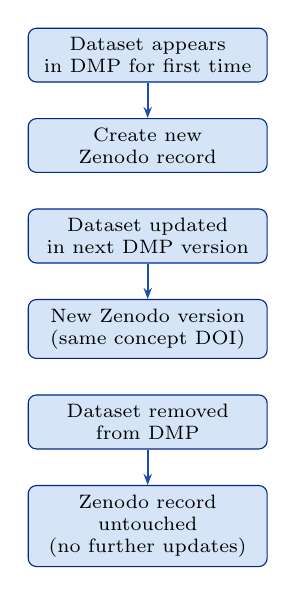
\begin{tikzpicture}[
        font=\scriptsize,
        box/.style={draw=crisnavy, fill=crislight, rounded corners=3pt,
                    text width=2.8cm, align=center, minimum height=0.65cm},
        arr/.style={-{Stealth[length=4pt]}, cristeal, thick},
      ]
        \node[box] (new)  {Dataset appears\\in DMP for first time};
        \node[box, below=0.45cm of new] (create) {Create new\\Zenodo record};
        \node[box, below=0.45cm of create] (known) {Dataset updated\\in next DMP version};
        \node[box, below=0.45cm of known] (ver)   {New Zenodo version\\(same concept DOI)};
        \node[box, below=0.45cm of ver]   (drop)  {Dataset removed\\from DMP};
        \node[box, below=0.45cm of drop]  (keep)  {Zenodo record untouched\\(no further updates)};
        \draw[arr] (new)   -- (create);
        \draw[arr] (known) -- (ver);
        \draw[arr] (drop)  -- (keep);
      \end{tikzpicture}
  \end{columns}
\end{frame}

\begin{frame}[fragile]{State tracking: \texttt{zenodo\_state.json}}
  Committed alongside \texttt{dmp.json} in the project repository.\\
  Maps \texttt{dataset\_id.identifier} $\to$ Zenodo concept DOI.

  \vspace{0.3cm}
  \begin{columns}[T]
    \column{0.47\textwidth}
      \begin{lstlisting}[style=yaml, caption={After first release}]
{
  "https://doi.org/10.5281/zenodo.AAAA":
    "10.5281/zenodo.AAAA",
  "https://github.com/myorg/proj/ds-B":
    "10.5281/zenodo.BBBB"
}
      \end{lstlisting}
      \vspace{0.2cm}
      \footnotesize Auto-committed by the pipeline bot after each
      successful release. No manual editing required.

    \column{0.50\textwidth}
      \textbf{Decision logic at publish time:}
      \vspace{0.2cm}
      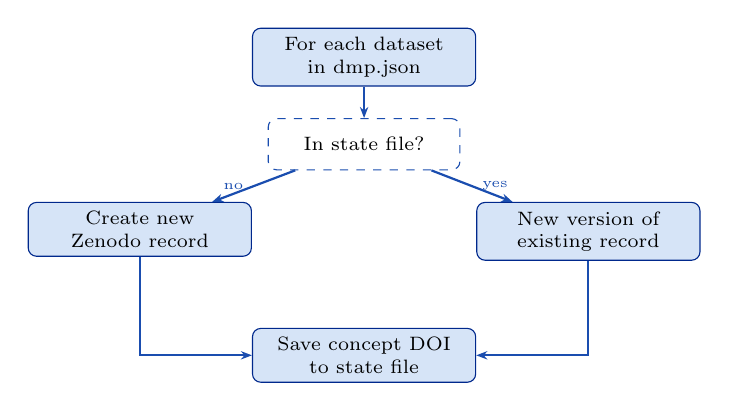
\begin{tikzpicture}[
        font=\scriptsize,
        node distance=0.4cm,
        box/.style={draw=crisnavy, fill=crislight, rounded corners=3pt,
                    text width=2.6cm, align=center, minimum height=0.65cm},
        dec/.style={draw=cristeal, fill=white, rounded corners=3pt,
                    text width=2.2cm, align=center, minimum height=0.65cm, dashed},
        arr/.style={-{Stealth[length=4pt]}, cristeal, thick},
      ]
        \node[box] (each) {For each dataset\\in dmp.json};
        \node[dec, below=0.4cm of each] (known) {In state file?};
        \node[box, below left=0.4cm and 0.2cm of known]  (cre) {Create new\\Zenodo record};
        \node[box, below right=0.4cm and 0.2cm of known] (upd) {New version of\\existing record};
        \node[box, below=2.0cm of known] (save) {Save concept DOI\\to state file};
        \draw[arr] (each) -- (known);
        \draw[arr] (known) -- node[left,font=\tiny]{no}  (cre);
        \draw[arr] (known) -- node[right,font=\tiny]{yes} (upd);
        \draw[arr] (cre)  |- (save);
        \draw[arr] (upd)  |- (save);
      \end{tikzpicture}
  \end{columns}
\end{frame}

%==============================================================================
\section{Institution adoption}
%==============================================================================

\begin{frame}[fragile]{Adopting fair-publish --- three steps}
  \begin{columns}[T]
    \column{0.48\textwidth}
      \textbf{Step 1 — Org-level setup (once)}
      \begin{itemize}
        \item Add workflows to \texttt{ORG/.github}
        \item Commit \texttt{fair-policy.yml}
        \item Store \texttt{ZENODO\_TOKEN} as org secret
      \end{itemize}

      \vspace{0.25cm}
      \textbf{Step 2 — Per project (minimal)}
      \begin{lstlisting}[style=yaml]
# .github/workflows/publish.yml
on:
  release:
    types: [published]
jobs:
  publish:
    uses: MY-ORG/.github/
      .github/workflows/
      fair-publish.yml@v1
    with:
      dmp_path: dmp.json
    secrets:
      zenodo_token:
        ${{ secrets.ZENODO_TOKEN }}
      \end{lstlisting}

    \column{0.48\textwidth}
      \textbf{Step 3 — Branch protection (governance)}\\[4pt]
      \begin{itemize}
        \item Require \textit{Validate maDMP} status check
        \item Apply via org-level Ruleset $\to$ propagates\\
              to all project repos automatically
      \end{itemize}

      \vspace{0.3cm}
      \begin{block}{What the PI sees}
        \begin{enumerate}
          \item Edit DMP in institutional tool
          \item Tool pushes \texttt{dmp.json} to GitHub
          \item Validation result visible in pull request
          \item PI clicks \textit{Create release} in GitHub UI
          \item Zenodo records appear automatically
        \end{enumerate}
      \end{block}
  \end{columns}
\end{frame}

%==============================================================================
\section{Demo}
%==============================================================================

\begin{frame}[fragile]{Running the pipeline locally}
  \texttt{simulate\_release.py} reproduces the full PI release cycle against
  the Zenodo sandbox --- no GitHub repository or production credentials needed.

  \vspace{0.3cm}
  \begin{lstlisting}[style=shell]
# Install the package
pip install fair-publish

# Validate only (fast feedback)
fair-publish validate example/dmp.json --policy example/policy.yml

# Full simulation: validate + publish to Zenodo sandbox
python simulate_release.py \
    --dmp    example/dmp.json \
    --policy example/policy.yml \
    --release-tag v1.0.0

# Output:
# == Step 1: Validate maDMP ==
# DMP: Longitudinal cohort study of metabolic biomarkers
# Datasets: 1   Errors: 0   Warnings: 0
# PASSED
#
# == Step 2: Publish datasets ==
#   [created] Metabolic biomarker dataset ... -> 10.5281/zenodo.XXXX
#
# State written to: example/zenodo_state.json
  \end{lstlisting}
\end{frame}

\begin{frame}[fragile]{Validation report in GHA}
  The step summary written to the GitHub Actions UI after each push:

  \vspace{0.3cm}
  \begin{lstlisting}[style=yaml]
## FAIR Validation Report
✅ PASSED — 0 errors, 1 warning

### Dataset: Metabolic biomarker dataset — cohort wave 1-5
| Rule                          | FAIR       | Status | Message              |
|-------------------------------|------------|--------|----------------------|
| Creator ORCID present         | F1, A1     |   ✓    | OK                   |
| License present and recognized| R1.1       |   ✓    | OK                   |
| At least one keyword          | F2         |   ✓    | OK                   |
| Description length            | F2, R1     |   ⚠    | 198 chars; min 150   |
| Access rights stated          | A1         |   ✓    | OK                   |
| Dataset identifier present    | F1         |   ✓    | OK                   |
  \end{lstlisting}
\end{frame}

%==============================================================================
\section{Summary}
%==============================================================================

\begin{frame}{Summary}
  \begin{columns}[T]
    \column{0.52\textwidth}
      \textbf{What fair-publish provides:}
      \begin{itemize}\setlength\itemsep{3pt}
        \item Pluggable rule protocol --- built-in FAIR rules
              + institution domain rules
        \item YAML policy config at org level, inherited by all projects
        \item Per-dataset lifecycle tracking (\texttt{zenodo\_state.json})
        \item Two-workflow GHA design: validate on push,
              deploy on release
        \item Git tags for publication status history
        \item CLI for local validation and sandbox simulation
      \end{itemize}

    \column{0.45\textwidth}
      \begin{alertblock}{Assumptions \& scope}
        \begin{itemize}\setlength\itemsep{2pt}
          \item DMP authoring tool is external
          \item Repos owned by institution
          \item Branch protection configured org-wide
          \item Metadata only (no data file upload)
        \end{itemize}
      \end{alertblock}
      \vspace{0.3cm}
      \begin{block}{Code}
        \footnotesize
        \url{https://github.com/irycis/fair-publish}\\[4pt]
        \texttt{pip install fair-publish}
      \end{block}
  \end{columns}
\end{frame}

{\setbeamercolor{background canvas}{bg=crisnavy}
\begin{frame}[plain]
  \begin{tikzpicture}[remember picture, overlay]
    \fill[cristeal] (current page.south west) rectangle +(\paperwidth, 1.2cm);
    \node[anchor=west, inner sep=6pt]
      at ([yshift=0.6cm]current page.south west)
      {
\includegraphics[height=0.9cm]{uah-logo-white.png}};
  \end{tikzpicture}
  \vspace{1.5cm}
  \begin{center}
    {\LARGE\textcolor{white}{\textbf{Questions?}}}\\[0.6cm]
    {\normalsize\textcolor{crislight}{\texttt{msicilia@uah.es}}}\\[0.4cm]
    {\small\textcolor{crisaccent}{\url{https://github.com/irycis/fair-publish}}}
  \end{center}
\end{frame}
}

\end{document}
